% !TEX root = ../thesis.tex
\chapter{Conclusion and Future Work}
\label{capitolo8}
\thispagestyle{empty}

We can see this thesis as a proper journey, in which we learnt a lot about the users and data that populate social networks, and how they can be tricky to deal with.
The legacy of our work is a tool that can be used by anyone and that can prevent undesired or unlucky interactions with potentially harmful bots on Twitter.

The development of such tool doesn't imply that perfection has been reached, not even at the last step of this journey. We are aware of the limitations our work is subject to, due to the limited time we could invest and to the lack of experience in this field, experience that we have grown, by cleaning and processing these data and by trying to give them meaning, in terms of empirical considerations. 

This chapter summarizes the obtained results, as well as the weaknesses faced and the possible future extensions that could strengthen the work done so far.

\section{Summary and Lessons Learned}
The overall considerations can be summarized along the main steps involved in the thesis development.

\begin{itemize}
\item[\PencilRight] We had to face the challenge of inserting a new piece of research into the prolific puzzle of social bots detection. We studied the work done in this field and decided to go deeper inside the classification methods available so far. It wasn't easy to make us space inside research works, especially considering the time needed to gather the proper amount of data, for this kinds of purpose. The job was challenging and we tried to exploit the time and the tools we had, to give the best contribution to the research as possible. We are pleased with the results obtained, in terms of dataset creations and tools developed. Obviously, some limitations came to visit, starting from the timespan of the data observations, moving forward with the computation power we invested, and so on.
\item[\PencilRight] Our methodology involved the data collection, whose required effort was one of the biggest of the entire project. The main - and the first - issue faced, indeed, regarded the data itself. We did not have a custom dataset to draw samples from. We needed five different targets for our classifiers, because five were the account types we wanted to focus on. 

We followed several leads, in order to build a proper dataset for the multiple classes classifiers, and to enrich the training set of the binary model. After all the data were clean and homogeneous, we crafted useful features to support the decision boundaries among targets. Multiple models were created and combined into an execution pipeline. They were selected and enhanced by evaluating their performance scores, with test sets coming from our datasets. 
At the end of the whole process, an online web application was build to wrap the final prediction Python script. We encapsulated it into a client/server paradigm, in order to be available to everyone.

\item[\PencilRight] During the stages needed to complete our work, we learned lots of things about models, tools, methodologies and related works. However, the most important thing we have seen is the significance of the data. Data plays the leading role in a data science project, without a wide, consistent, stratified and concept-representative dataset, the models won't be able to approximate the actual targets correctly. This is the main issue met with our approach.
We gathered a nice amount of stratified data, but the problem is inherent to that stratification. Every class differs from the others with significant distinctive traits, leading to a relatively effortless model selection. Our classifiers fits our data very well, with pleasing metric scores, but are they really capable of generalizing over unseen samples?\\
What happens when we feed our classifiers with a brand new, borderline entry, without characterising marks? Here the nature of the datasets used emerges.

We don't have much instruments to be compared with ours, since the available works put the effort into bots and humans detection. Lately in this chapter, we provide a wide scale projection of the Twitter population, and use the outcome to compare our work with other public studies that made the same study on large numbers.
\end{itemize}


\section{Outputs and Contributions}
The contributions of our thesis can be summarized with three main points:

\begin{itemize}
	\item[\PencilRight] The construction and the release of a multi-class dataset, composed of 21,743 bot samples, labelled with four targets: \textit{NSWF} (\textbf{0}), \textit{News-Spreaders} (\textbf{1}), \textit{Spam-Bots} (\textbf{2}) and \textit{Fake-Followers} (\textbf{3}).
	The dataset was built following different approaches and assembling freely accessible data from previous researches, as discussed in Chapter \ref{capitolo3}.
	It is accessible for free at \url{http://botbuster.it/dataset}.
	
	\item[\PencilRight] The overall methodology followed to build our classification system. After the samples gathering, we studied how to build some features from raw data, in order to better describe the concept of the classification problem. Several models have been tested with raw settings and that led to a final pool of three multi-class classifier and a binary model.
	The bot-or-not Random Forest was build following part of the methodology used for Botometer, starting from the same training set, and then enhancing the data with newer samples. The performances of our model and Botometer have been compared, in order to have a reliable binary classifier to start our pipeline with.
	The second step involves the bot behaviour classifier. It is composed of three stacked models: a Random Forest algorithm fitted with the complete feature vector, a K-nearest neighbours model that considers only user data, without tweets meta-data, and a Naive Bayes text-classifier which, complementarily to the KNN model, classifies bots by reading their tweets only. The models stacking is performed with a Logistic Regression meta-model that takes as input the outputs of the previous algorithms, and performs the final probability prediction. Such stacking model is trained with bots data only and it is used to better defining the bot behaviours, repartitioning the probability that an examined account is a bot, according to the bot-or-not model. This prediction pipeline was tested with a 10-fold-crossvalidation, peaking a 0.987 score in the F1 measure, 0.987 of Precision and 0.986 of Recall metrics.
	
	\item[\PencilRight] \textbf{BotBuster}, the web application. It is an instrument aimed to classify every Twitter user, with no discriminations about their tweeting activities. It is the implementation of the methodology discussed in our thesis. The tool provides ``soft`` classifications, which means that the outcome returned by the engine is a probability vector, and not a specific target. It assigns, to the examined account, the membership likelihood to each target involved in our study.
	The prediction rendered with vertical bars contains probabilities for NSFW, News-Spreaders, Spam-Bots, Fake-Followers and Genuine category.
	BotBuster is accessible for free at \url{http://botbuster.it} for testing.
	
	\item[\PencilRight] A wide scale projection for the Twitter population.
	We provide an estimation of the bots distribution on the social network, sampling and classifying 12k random accounts. The process and the results are discussed in the following section.
\end{itemize}

In addition with the usefulness provided to the internet users, with the development of such instrument, we hope that the study we made could become a starting point for those who are interested in building more sophisticated tools for automatic recognition of social bots, and the identification of their potentially harming behaviours, even in cross-platform environments.

\section{Projection on wide scale}
Being now able to automatically classify Twitter accounts into genuine users or different types of bot accounts, we wanted to give and estimation about the bots distribution over the full Twitter population. In order to be able to do that, we needed to sample unseen users from the social network and to classify them with our tool.
Starting from 200K randomly generated IDs, within a feasible ranges of numbers, we checked each identifier with the Twitter APIs, to verify if they were actually bounded to existing accounts.
This filtering process left us with just 12,616 retrieved profiles.
Then, we analysed every one of those users with BotBuster, and the results are shown in Figure \ref{fig:projection}.
\begin{figure}[htp!]
	\begin{center}
		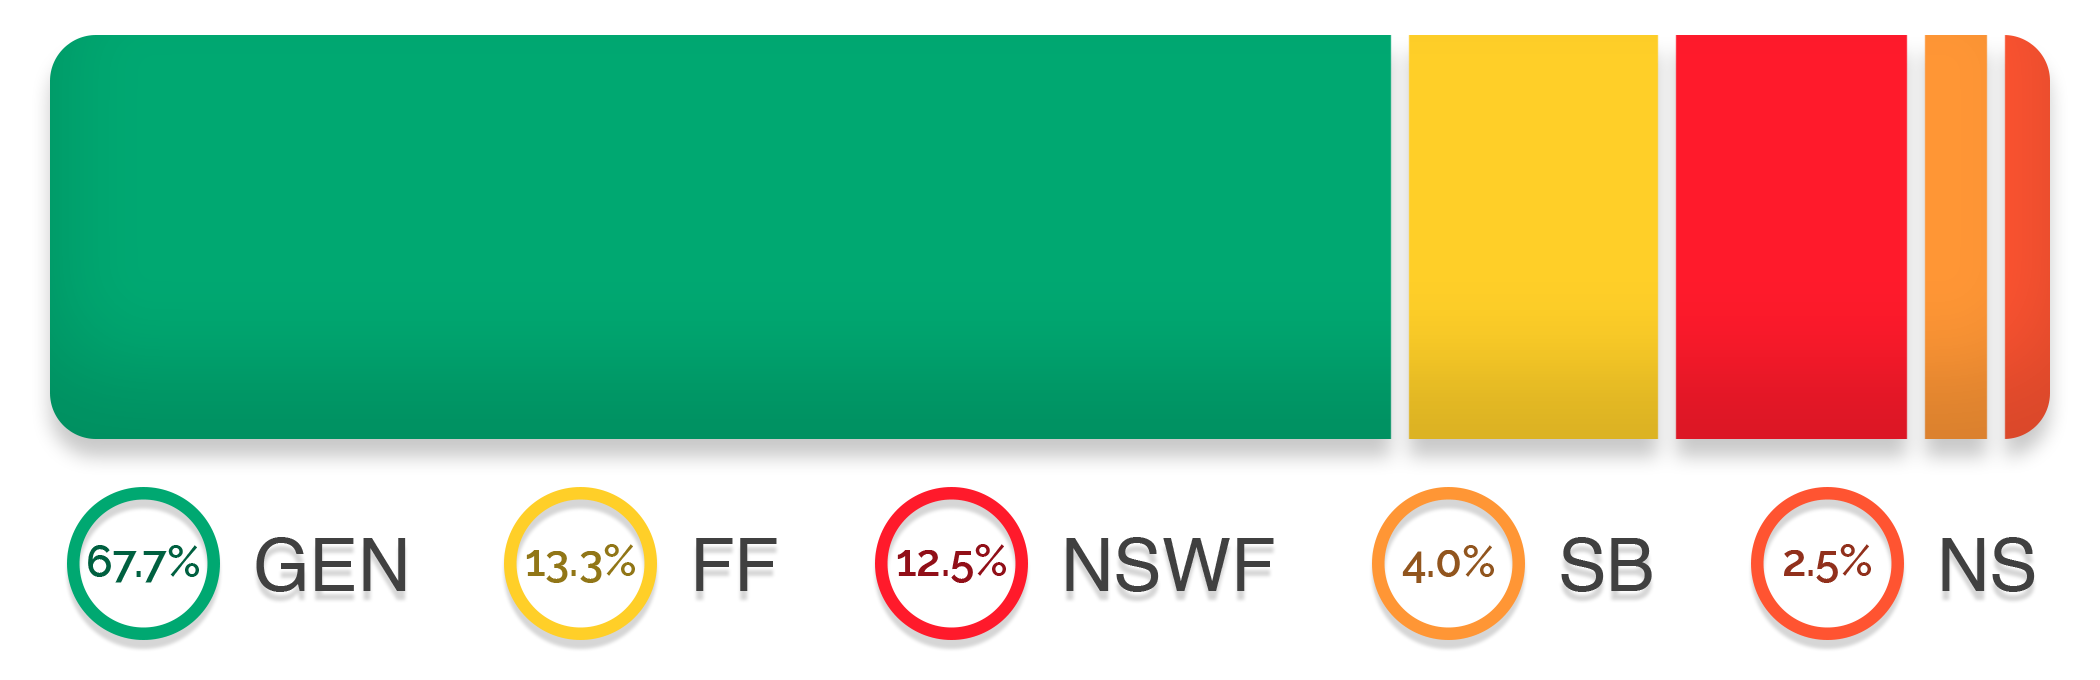
\includegraphics[width=\columnwidth]{chapter8/figure/projection.png}
	\end{center}
	\caption{Projection on Twitter population}
	\label{fig:projection}
\end{figure}

What we can infer from this chart is that the most representative category of accounts is the Genuine one.
It is reasonable to assess that the legitimate accounts populate Twitter for the most, but, according to our analysis, there may be even up to twice as many bots on Twitter as identified in by Varol et al. \cite{Varol}. The researchers of that paper claim to have sampled 14Mln accounts and to have found a bot percentage that is up to 15\% of the entire population.
The classification of such amount of users would have taken us an incredible timespan to be executed, since the average prediction takes 12 seconds to be computed.
One other thing that may have led us to different results is that we took into account totally random samples, which means including also inactive users.
Users are marked as active if they logged at least once into the system in the last six months. According to Twitter, the current population of active users is composed of about 326Mln of accounts \ref{fig:active}. We managed to reach 12K profiles and lots of them are most likely inactive, given the high ratio of Fake-Followers found with BotBuster. Fake-Followers are is characterized by low tweeting activity, along with other factors, such as the number of accounts that follow them. BotBuster seems to classify inactive users as Fake-Followers, because they usually lack tweets. It is a limitation imputable to the nature of the training sets, since we didn't have enough samples with such low activity, marked as legitimate.

What really emerged from this experiment is the high ratio of inactive users found by randomly sampling Twitter accounts. They have been distributed among Genuine, Fake-Followers and NSFW, depending on two factors: their level of interaction and their profile pictures.
Each of these inactive users are characterized by a very small number of tweets, but the ones which have no tweets, no followings, followers, custom profile pictures or likes have been marked as genuine by the tool. The ones that have at least one of those aforementioned fields with non-empty value are classified according by the rules of our models. The issue in this approach is represented by the Inception module for the image features computation. If the neural network fails in classifying a picture correctly, the examined user could be marked as NSFW, even with an almost-complete lacking of interactions, just by looking at her profile photo. This behaviour explains the high ratio for both Fake-Followers and NSFW classifications, with the retrieved samples.

\begin{figure}[t!]
	\begin{center}
		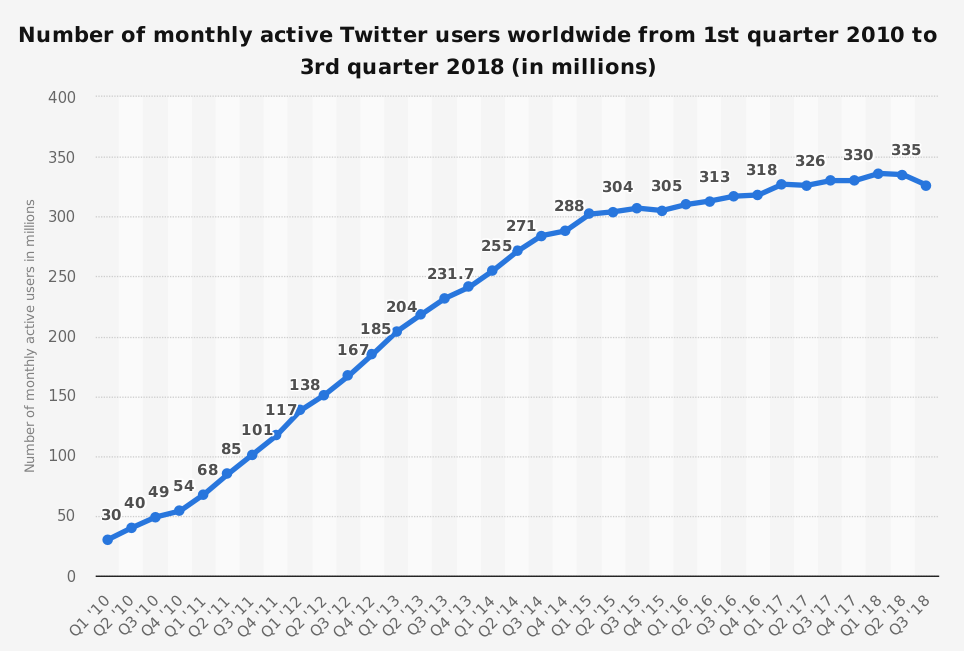
\includegraphics[width=\columnwidth]{chapter8/figure/active_accounts.png}
	\end{center}
	\caption{Number of monthly active Twitter users worldwide\\
	Release date: October 2018\\
	\url{https://www.statista.com/statistics/282087/number-of-monthly-active-twitter-users}}
	\label{fig:active}
\end{figure}

\section{Limitations}
As said before, we met several limitations in our thesis, and they came both from external factors and internal choices that affected the final results.

The external factors are, for the most, the time and the computational power.
We can impute to the data the most limitations, but the fact is that, with the right amount of time, we could had collected a better dataset, exploiting different and non tested methodologies. For instance, we could have used social honeypots, crafted to trigger specific kinds of bots, maybe capturing more diversity in our data, involving new waves of social bots, as well as more institutional accounts, like editorial or politics users. We lacked verified profiles in our training sets, we think that adding more accounts with the verification mark could be helpful to extend the legitimate behaviour's spectrum that we have analysed. We can observe the struggle of our classifiers, when it comes to such verified accounts.

Even the other categories could have been extended with borderlines accounts, in order to make more flexible decisions. Once again, it is a matter of time, mostly.
The computational power didn't represent a major issue, but the lack of such power led to a general slow-down of the work, which denied us the possibilities to do further experiments, like the ones described above.
The calculations of some features, like the extrinsic attributes and the image classification, required lots of time, with the tools we had. Some algorithms had to be run for hours, entire nights or days. The Grid Searches used to find the best hyperparameters configurations took us much time, and they have been repeated very frequently. Every little change, every little different choice, brought us to recalculate the best models' settings, which means Grid Searching over the parameters space, repeatedly.
It could have been faster with cloud computing solutions.

When it comes to internal choices, we have to start with something we lacked, especially at the beginning of this journey: the experience.\\
Inexperience made us chose some moves that, in operative terms, wasted precious time.
For instance, the programming skills with Python and the machine learning frameworks weren't fulfilling the necessities, at the first stages of the work.
We spent a lot of time struggling with programming paradigms and handling the dataset, with information losses that forced us to repeat basic operations and restore entire processes.
These limitations have been mitigated with the experience on practical coding, and the entire workflow had a speed-up, as the time passed.
Some inexperience-driven limitations, that not necessarily represented a bad handling of the time, were the attempts that revealed to be failures, but that made us learn something more about methods and contexts.
For instance, one of the first hands-on tries on the data was to apply an unsupervised labelling to a binary dataset, in order to catch useful patterns and to simplify the targeting process. By that time, we thought that there weren't other ways but handling labelling the datasets. Fortunately, and thanks to that unlucky approach, we found out new ways to collect the labelled data.

Due to inexperience, some choices we made, when we were building the first models, have been rushed, in comparison with the decision taken once the overall structure was clear. Sometimes, we went back to old decisions and we tried different possibilities, in order to better adjust some features to a pipeline, instead that to the previous stacking method. This revisiting process took much time, and we are aware that there are still things that could be refined better.

For instance, the extrinsic features have been passed under different tests, before choosing the final configuration. This is how we arrived to totally disjointed dictionaries. But we did not play with the number of initial words retrieved, taking 1000 as fixed (older versions had less words). We could have applied empirical methods to choose the right amount of terms to consider.

Also, we did not consider language-dependent features. This process was a consequence of the first adaptations to the data retrieved. We were gathering only American accounts, and the textual features were initially thought to fit that language.
With the extension of the dataset, especially with the Fake-Followers category, we introduced different parts of the world in our data, with their languages. This made the data heterogeneous, without adjusting the attributes. Geolocalization is not taken into account as a feature, as well as the nationality. 

Some attributes were deleted after observing a large number of missing values. One example is the colour chosen by the user to fill the profile tile (a rectangular-shaped space that lies under the profile picture and that can be filled with photos or plain colours). Since it is represented as a string (RGB hexadecimal code), in order to be handled by the algorithms we built, it should have been encoded with techniques as One-Hot encoding, that would have made the number of features explode. We could have found better way to handle the missing values and the encoding of such features.

Another thing that could have been done, and that we actually considered, is sentiment analysis on tweets. We could have relied on external services, but sticking to a low number of calls for the APIs, because these are paid services that offer limited free solutions. Implementing our own sentiment classifiers would have been expensive, in terms of time and effort. We preferred to spend that time to refine the features we already had and to add a classifier to the ensemble.

\section{Future Work}
Several things could be implemented by future works. The most important ones could be the dataset extension, as well as the detection of new targets.
Since we studied the Twitter platform, we stuck to a narrow range of harmful behaviours. This range could be extended with new classes to perform classifications on. Offensive bots, like the ones that incite to hate or racism, are outside the domain of our study, because we did not find a proper method to collect a reasonable amount of them. The missing sentiment analysis discouraged us to identify the level of hate or offensive contents in tweets. This insertion could make the target space wider.

Another useful work that could be done is the evolving training of our models. It could be implemented a way to receive trusted feedbacks over the performed classifications. Such indications, along with the classified sample, could feed the models by adding that entry to our training set, with the indicated target. Obviously, feedbacks should be trusted and not biased. A heuristic method to choose which feedback consider should be implemented too, as well as reinforcement learning algorithms, to improve the evolving training.

A more sophisticated image recognition system can be included. NSFW category is a well defined sphere of the bots ecosystem, it would be very easy to detect it with the right instruments. By now, we have an Inception convolutional neural network, used to compute two features bounded to the images. It would be interesting getting some insights from video contents too, in feasible computation time. The image features aren't 100\% accurate, due to the validation error found and to the data used to fit the network. It can be improved, with more and diversified samples. The time needed to process ten images discourages us to look for more media content to analyse. It would be a robust support to be able to lookup more tweets with media contents embedded.

Some features that look outside the user's box could be added, like the ones which get clues from the user's network, from her friends or the accounts that quote and retweet her. We had our focus on the user's routine, with meta-data about her relationships, but we don't get inside those interactions.                



